
\documentclass[12pt]{article}
\usepackage{hyperref}
\usepackage{graphicx}
\usepackage{float}
\pagenumbering{arabic}
\graphicspath{ {./images/} }
\begin {document}

\title {AirSync}
\author {Robert Durham\\
	\texttt{durhamrj@gmail.com}}
\date {\today}
\maketitle

\section{Introduction \& Motivation}
Many portable devices have become a part of our everyday lives impacting work as well as our home lives and the way we travel. Most of these devices have their own unique means of transferring media and documents. All of these devices can access the internet via some means, e.g. WiFi or cellular network. I will use my situation as an example, between myself and my wife we have at least eight different devices that we like to access music libraries, documents, photos and videos from:

\footnotesize
\begin{center}
\begin{tabular}{|l|l|l|}
\hline
	\textbf{Device} & \textbf{Description} & \textbf{Connectivity}\\
\hline
	Desktop PC & Linux & Wired(Home)\\
\hline 
	Home Theater PC & Linux & Wired(Home)\\
\hline
	Laptop(Mine) & Windows 7/Linux & WiFi\\
\hline
	Laptop(Spouse) & Windows XP & WiFi\\
\hline
	Motorola Droid 4(Mine) & Android 4 Phone & 4G \& WiFi\\
\hline
	Motorola Droid 3(Spouse) & Android 2.3 Phone & 3G \& WiFi\\
\hline
	Nexus 7 & Android 4 Tablet & WiFi\\
\hline
	Kindle Fire HD & E-Reader/Tablet (Android 4 based) & WiFi\\
\hline
\end{tabular}
\end{center}
\normalsize
Several `Cloud' services have offered means to maintain and provide access to media and documents via the internet, e.g. Apple iCloud, DropBox, Asus WebStorage, Ubuntu One. All of these have limited storage, cost money to expand that storage, and don't support all necessary devices. These issues are outside of the fact that these require trusting your personal data to a $3^{rd}$ party. DropBox and Ubuntu One support almost all of these devices, but transferring large media files through internet is slow. What if there were a solution to easily synchronize media/files through your home network, yet still allow access to these files through the internet without relying on the privacy policy of a $3^{rd}$ party provider? Some open source solutions can help in desktop/laptop situations, but not with mobile devices.

\section{Goal}

The goal of this project is to provide a means to easily synchronize files between multiple types without relying on $3^{rd}$ party services to protect sensitive data. In order provide a replacement option for services like dropbox, AirSync must provide a means to access files remotely through the internet.

\section {Use Cases}

Their are three types of devices and two types of connections used to depict each of the use cases.  The three types of devices are static PC, mobile PC and mobile device.  The two types of connections are local and internet connected. A localized connection refers to the situation where the devices do not need to utilize internet bandwidth to transfer data.  Local connections are typically at least 54 mb/s where as most internet connections in 2010 averaged 3.7 mb/s\footnote{http://arstechnica.com/telecom/news/2010/01/us-broadband-still-lagging-in-speed-and-penetration.ars}. 54 mb/s is the theoretical limit of 802.11g wireless networking protocol. Hotels have notoriously slow internet connections.

\begin{enumerate}
\item Synchronize files between server and devices on local network
\item Manage Android file system from static or mobile PC on local network
\item Download/Upload files between server and Android Device or Mobile PC via internet connection
\end{enumerate}

\section{Design}

AirSync will provide the means to synchronize files between any Windows, Linux and Android devices. It will include the following three software components: 
\normalsize
\begin{center}
\begin{tabular}{|l|p{7.5cm}|}
\hline
	\textbf{Component} & \textbf{Description} \\
\hline
	Service 
	& Runs as system service or daemon on server and client PCs. Acts as Server and/or Client depending configuration. \emph{A client needs to be capable of becoming a server\ldots} \\
\hline 
	Service Configuration UI & Graphical User Interface that will monitor status and change settings with AirSync Service on PCs. Will also provide remote management of files on Android devices.\\
\hline
	Android Client Application & Activity App that will provide the user with a choice of two operating modes. One mode will allow remote management of the android devices memory space from the Service Configuration UI. The second mode will allow the Android user to browse the files available from the server and select files to download.\\
\hline
\end{tabular}
\end{center}
\normalsize
All application components will be developed in Java to maximize code re-usability and portability between platforms. \emph{Android}\footnote{http://www.android.com/developers/} is essentially any embedded Linux environment with a specialized Java Virtual Machine. If Android specific code sections are properly abstracted into separate Java Classes, the large majority of the android client code will be re-usable with the PC application. The Integrated Development Environment (IDE) will be \emph{Eclipse}\footnote{http://eclipse.org/} with the Android Developer Tools(ADT) addons. \emph{Git}\footnote{http://git-scm.com/} will be used for source versioning control with the git server being hosted on \emph{github.com}\footnote{https://github.com/durhamrj/AirSync}. This project will not include the development of an AirSync application for \emph{Apple IOS}\footnote{https://developer.apple.com/devcenter/ios/index.action}. The development environment for IOS only supports Mac OS X. The IOS development language is a managed C++, much of the code would need to be ported and I do not have access to a Mac, so I have exclude support, for now. 

\subsection{Service Design}

\begin{itemize}
\item Server side component, provides remote access to files based on system configuration
\item Tracks initialized devices and associated unique ids
\item Communicate transfer files and status 
\end{itemize}

\subsection{Service Configuration UI Design}

\begin{itemize}
\item Graphical interface to service for configuration and status monitoring
\item Enable access to certain files and folders.  Potentially on a per device basis(Access Restrictions).
\item Log remote transfers
\end{itemize}

\subsection{Android Client Application Design}

\begin{itemize}
\item Provide client file synchronization with service
\item Allow remote file selection for download 
	\begin{itemize}
	\item when not on localized network
	\item user selectable
	\end {itemize}
\item Provide remote file system management to service
\end{itemize}

\subsection{Source Code Organization}
\begin{center}
\emph{\textbf{This section is being updated as the project progresses.}}\\
\end{center}
The source code and build files for this project can be found at \emph{http://github.com/durhamrj/AirSync}. The Service and Service Configuration UI share a common Eclipse/Java project. The components are separated by the package structure within this project. The  folder structure of the project is as follows:

\begin{center}
\begin{tabular}{|l|p{7.5cm}|}
\hline
	\textbf{http://github.com/durhamrj/AirSync} \\
\hline
	AirSyncServer/ 
	& Cross Platform Java application for Desktop and Laptop computers\\
\hline 
	RemoteSync/
	& Android application source code and project files\\
\hline
	docs/
	& Contains documentation for project include latex source for this PDF\\
\hline
	README.md
	& An autogenerated file created by github\\
\hline
\end{tabular}
\end{center}

\subsubsection{AirSyncServer Project Structure}

\begin{figure}[H]
\center
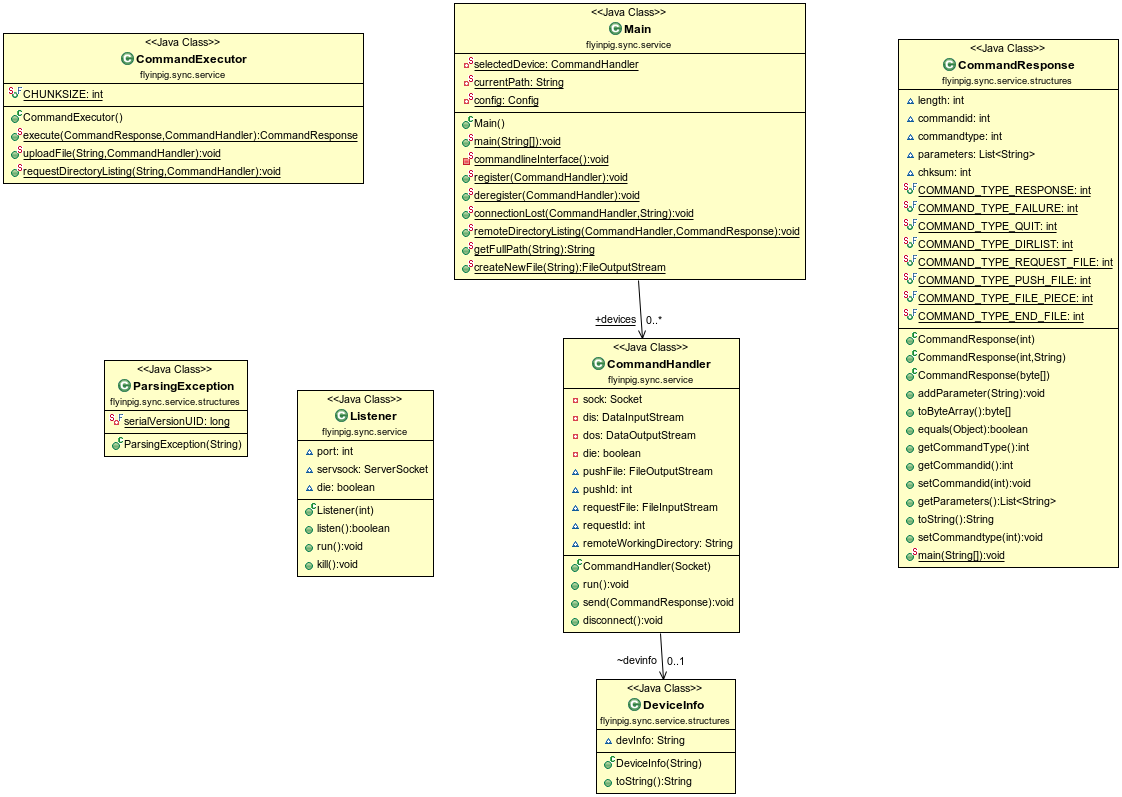
\includegraphics[width=1\textwidth]{class-diag.png}
\caption{AirSyncServer Class Diagram}
\end{figure}

\begin{center}
\begin{tabular}{|l|p{7.5cm}|}
\hline
	\textbf{AirSyncServer Source} \\
\hline
	\emph{\textbf{flyinpig.sync.service}}\\
\hline 
	CommandHandler.java
	& Handles socket IO with client connections as a separate thread\\
\hline
	Listener.java
	& Opens listening port in a thread and spawns new CommandHandler threads for each new incoming connection. New connections are tracked for display in the UI.\\
\hline
	Main.java
	& Singleton class. Includes the application main and fields/structures to track connection application state information.\\
\hline
	\emph{\textbf{flyinpig.sync.service.structures}}\\
\hline
	CommandResponse.java
	& Handles conversion of commands \& responses between Java objects and binary data to be transmitted over Socket IO. This was initially intended to use XML serialization, but due to a lack of android support the conversion is all manually coded in this file and uses not additional system libraries.\\
\hline
	DeviceInfo.java
	& Contains specific information about a device sent on initial connection. Used to hold information displayed within the UI to uniquely identify each device.\\
\hline
	ParsingException.java
	& Exception thrown by CommandResponse when errors occur parsing command \& responses.\\
\hline
\end{tabular}
\end{center}


\subsubsection{RemoteSync Project Structure}

The file structure in the Android project is largely made of generated files. I will only identify the files that I have manually modified as well as source code I have written. Many of the source files are identical between the AirSyncServer project and the RemoteSync Android project.\\

\textbf{Lines of Code by file:}\\
  255 ./flyinpig/sync/RemoteSyncActivity.java\\
  261 ./flyinpig/sync/ACommandExecutor.java\\
   14 ./flyinpig/sync/io/ParsingException.java\\
  199 ./flyinpig/sync/io/ClientThread.java\\
  224 ./flyinpig/sync/io/CommandResponse.java\\
  953 total

\begin{figure}[H]
\center
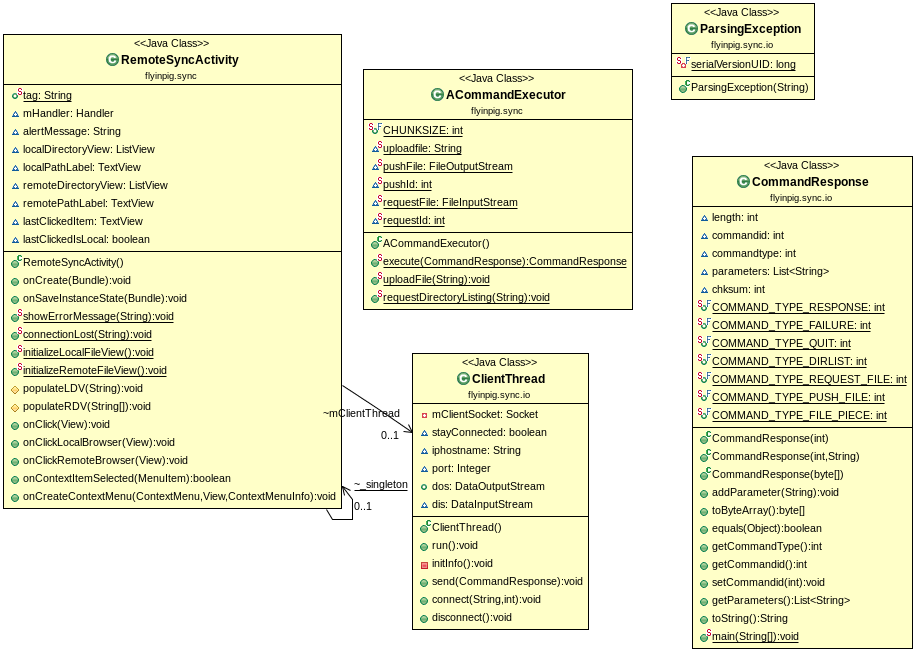
\includegraphics[width=1\textwidth]{android-class-diag.png}
\caption{RemoteSync Class Diagram}
\end{figure}

\begin{center}
\begin{tabular}{|l|p{7.5cm}|}
\hline
	\textbf{RemoteSync Source} \\
\hline 
	AndroidManifest.xml
	& This file is most importantly used to set application permissions.\\
\hline
	\emph{\textbf{flyinpig.sync}}\\
\hline
	RemoteSyncActivity.java
	& Main class for application. Monitors/Controls application view and state. Views are generated with a graphical interface in the android developement kit.\\
\hline
	ACommandExecutor.java
	& Handles CommandResponse objects and executes the associated commands. Acts as an abstraction Layer between ClientThreads networkIO and the UI components.\\
\hline
	\emph{\textbf{flyinpig.sync.io}}\\
\hline
	ClientThread.java
	& Handles Client Socket IO. Similar to CommandHandler but more specific to android threading and IO paradigm.\\
\hline
	CommandResponse.java
	& Handles conversion of commands \& responses between Java objects and binary data to be transmitted over Socket IO. This was initially intended to use XML serialization, but due to a lack of android support the conversion is all manually coded in this file and uses not use additional system libraries.\\
\hline
	ParsingException.java
	& Exception thrown by CommandResponse when errors occur parsing command \& responses.\\
\hline
\end{tabular}
\end{center}

\section{Using AirSync}

Two files are required to run AirSync. 
\begin{itemize}
\item \textbf{RemoteSyncActivity.apk} Android applicaton. This can be copied on any android device v2 or newer and installed. Acts as a client connecting to the AirSyncServer allowing for management and transfer of files on both the android device and the server.
\item \textbf{AirSyncServer.jar} This jar should be executable on any system with a properly installed Java Runtime Environment(JRE). I have tested this jar with both, openjre v7 and Oracle JRE v7. Though, I believe this jar will execute properly with JRE versions as old as v5.0, it has not been tested.
\end{itemize}

\subsection{AirSyncServer}

To run the AirSyncServer, copy the .jar file to the system you wish to run it on and ensure that a version of the java runtime is properly installed. Double clicking the jar file will execute the jar and a command prompt will open with the jar running. 

\textbf{Screenshots and specifics to come once I finalize the server component}

\subsection{RemoteSync Android App}
In order to install the user must go into the devices system settings. Typically, varying with device vendor, in either Security or Application settings there is an option to allow installation of applications of unknown source. This means that you are allowing the device to install applications that did not come from Google's android market or 'play store'.\\\\
Once the application has been installed, looking in the application tray on your device you should find the RemoteSync application. If it doesn't not appear in the application then the application was not properly installed. The following screen will appear on your device. All of these screenshots were taken within the android development emulator and the controls on the right hand side of the device screen can be disregarded.\\

\begin{figure}[H]
\center
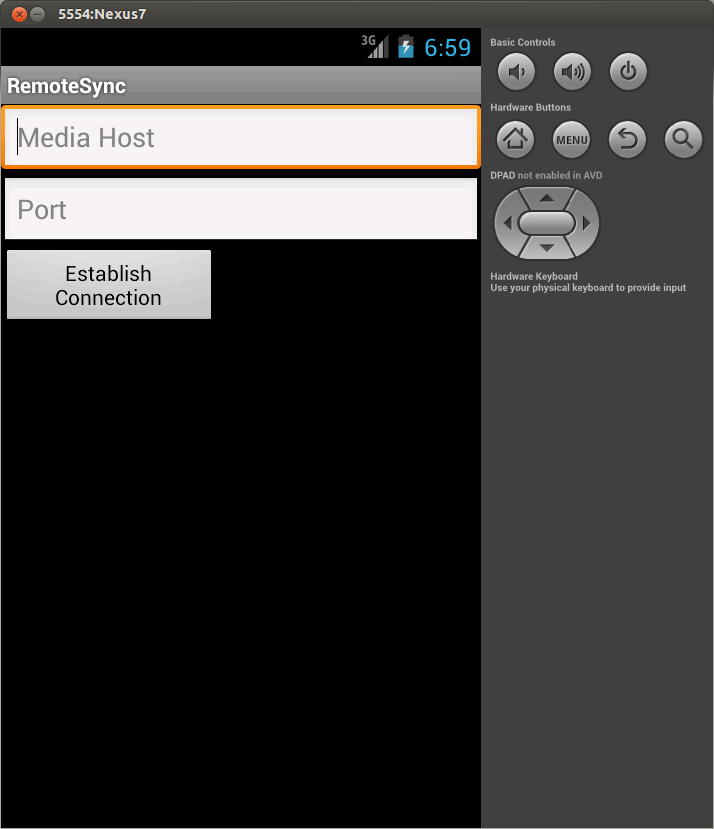
\includegraphics[width=0.6\textwidth]{android-main.png}
\caption{RemoteSync Initial View}
\end{figure}

In the first field 'Media Host' fill in the IP or host URL where your the server application is running. In the second field, fill in the tcp port that the server is configured to run on. Tap 'Establish Connection' to connect to the server. If the application fails to connect check your networking configuration, server firewall setting s and try again. Once the connection has been established the screen will change to a local device browser.

\begin{figure}[H]
\center
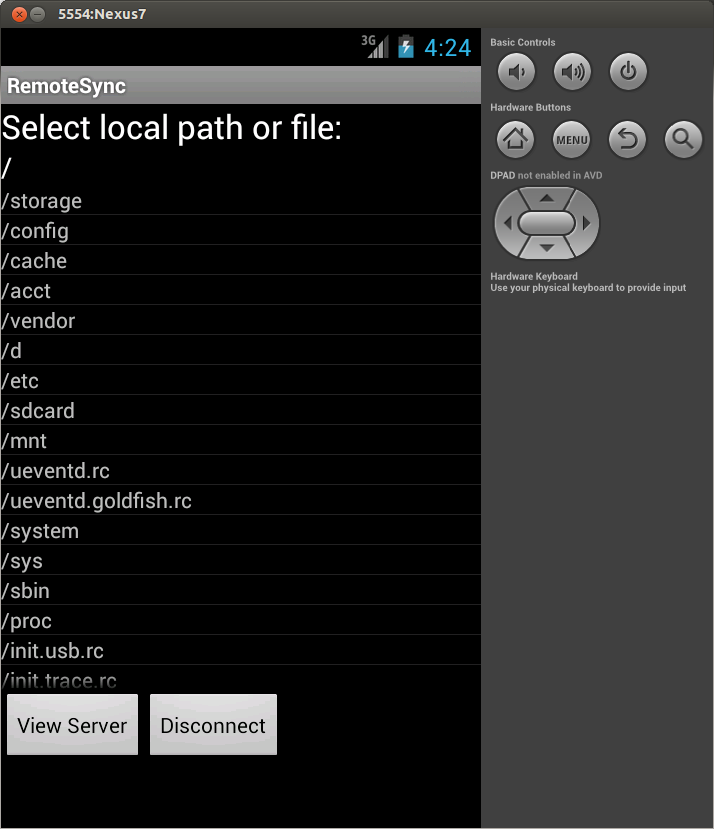
\includegraphics[width=0.6\textwidth]{local_browse_view.png}
\caption{RemoteSync Device File Browser}
\end{figure}

Tapping a folder will browse into that folder. Tapping a file will bring up a menu prompting to upload that file to the server. The upload will push the file the folder that the server is navigated to. On initial connection that folder is the root folder that the server is configured to allow access to. Tapping 'View Server' will switch to a remote view of the servers file system. Tapping 'Disconnect' will close the connection to the server and change the display back to the initial view. Tapping on the larger text that displays the current path that the browser is listing will browse to the parent folder.

\begin{figure}[H]
\center
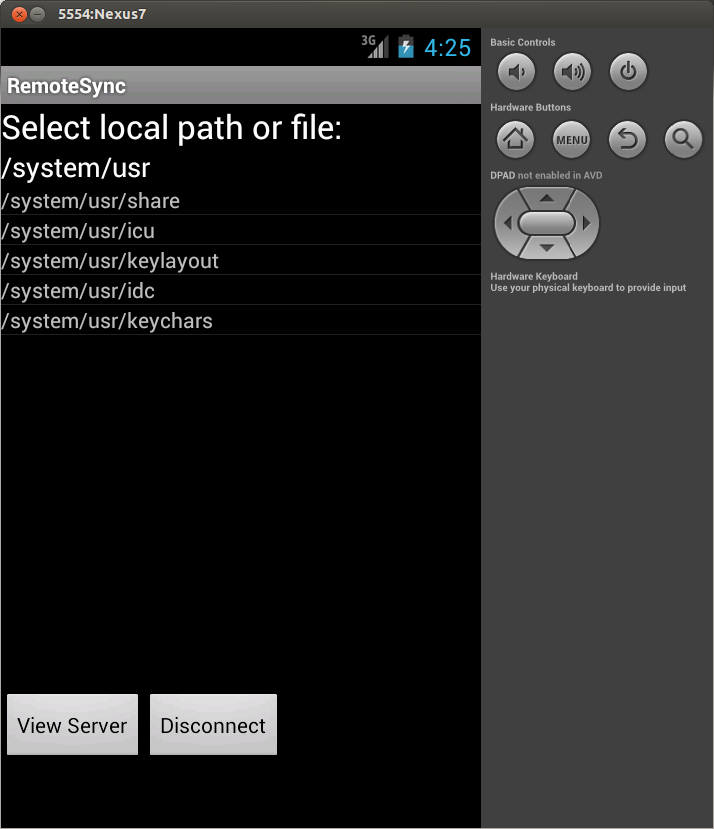
\includegraphics[width=0.6\textwidth]{deeper-browse-folder-view.png}
\caption{RemoteSync Browser Subfolders}
\end{figure}

\begin{figure}[H]
\center
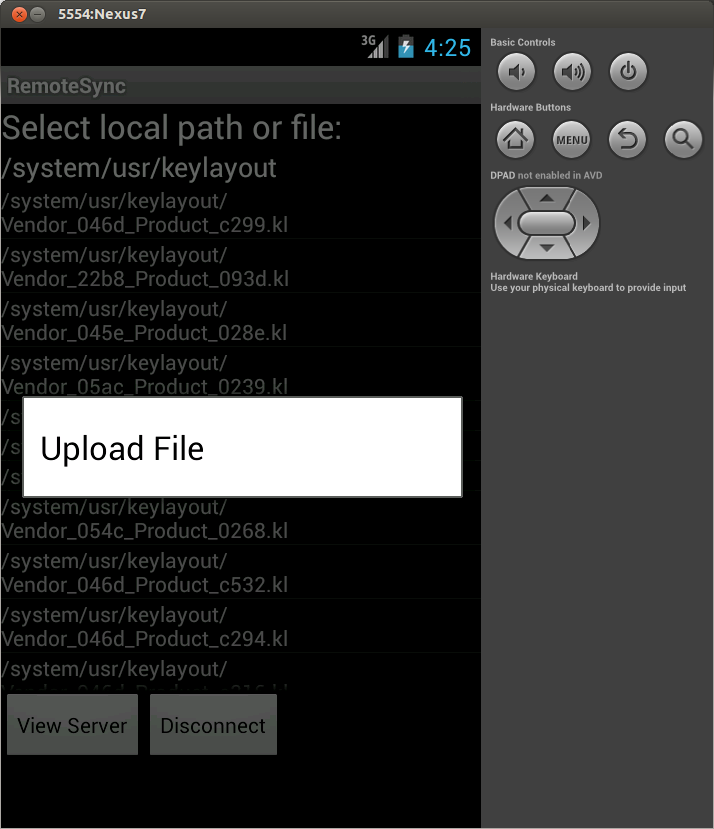
\includegraphics[width=0.6\textwidth]{upload-file.png}
\caption{RemoteSync Upload File Prompt}
\end{figure}



\section{Current State}
The project can be demonstrated to meet use cases 2 and 3.  Use case 1 has not been implemented because it will require an additional android project to run as a service and allow continuous synchronization.  This use case is far more complicated than I original expected, not only because of the addition project / application required but that it also requires continuous monitoring of the mobile devices power and networking state. Also, services cannot provide user interaction, the interaction needs to occur through an Activity. All configuration and status monitoring will also need to occur through an Activity.  In the Lessons Learned section I describe some specific pitfalls that can occur with a inexperienced android developer. This Activity / Service paradigm along with strict permissions is an example as well. I believe it would require double the effort already expended to develop the proper service and activity interactions to meet the desired usability.\\\\
In order to ensure the backend transfer code was stable and working well I have put off the user interface for the desktop version. My second reason for putting off the UI is that the publicly addressable server I use as an intermediary to transfer files doesn't not have a graphical interface. It is only accessible through SSH. I have been using this server for the majority of my testing and would be unable to test the UI on this system. All of the screen shots of shown in the 'Using AirSync' section are of the commandline interface I created to perform utilize all of the components. I intend to complete the UI component before releasing AirSync to the public. The commandline option will still be usable through a '-nogui' commandline flag when executing the jar.
\subsection{Desired Additional Features}
Besides the use case described above there are some features that have not been implemented in the project.
\begin{itemize}
\item \textbf{Visual Indicators \& Progress Bars:} Looking at it initially it would seem that adding progress bars to show on the android what is occuring. This will give the user confidence in knowing what exactly the application is doing and that a file transfer is actually happening and how long it will take.
\item \textbf{SharedPreferences:} Applications have a defined method for save instance state information when an application loses focus, but this is intended for running information. If an application is "Force Closed", by a user, the saved instance information will no longer exist. SharedPreferences provides a mechanism to store configuration information in a persisted Hash Table using key/value pairs. Similar to how the Windows Registry works the values can be stored as Boolean, String, or Integer values. Windows, unlike Android, also allows binary data and does not restrict access by other applications. 
\item \textbf{MediaStore:} Android provides specifc folder structures and tracking mechanisms for media files. The folder structure and location can vary from device to device. Using MediaStore provides a mechanism to manage media files and playlists from an application while abstracting the file system structure. The current implementation lets the user browse the file structure and select the media directories manually.

\item \textbf{Batch File Transfer:} Currently files can be transferred one at a time, but the user must wait for a file to transfer before queueing more file transfers. A queued transfer list and progress display would solve this problem.
\item \textbf{Access Control:} In order to prevent any device or any person from connecting to any server and accessing/manipulating files the software needs to implement user and/or device based access control. This feature should implement the Bell-LaPadula confidentiality focused access control model.
\item \textbf{Encrypted Communication:} Encrypting communications channels is necessary to protect the privacy of the files in transit across a network, whether wireless or wired. SSL is a very common standard implementation to enable encryption in most applications. SSL can be configured to utilize AES 256 bit encryption, which is NIST FIPS compliant.\footnote{http://src.nist.gov/publications/fips/fips197/fips-197.pdf}

\item \textbf{Historical Versioning:} Historical versioning would be useful in recovering overwritten files.  The most robust way to implement this feature is to incorporate a version control library for the server portion of the project.\footnote{http://svnkit.com/} Subversion is widely implemented, and most suited for this task. The merge functionalities of subversion will need to be disabled for this feature.
\end{itemize}

\section{Lessons Learned}

Before diving into the project development I want to discuss the documentation. This is the first time I have used \LaTeX  for documentation. I have very impressed by the versatility and consistency. Any time that I have lost learning its nuances while generating this documentation has likely made up for the time that I would have spent in Microsoft Word or OpenOffice trying to perfect the documents formatting.  It allows you to focus on writing the text and generating the content without being distracted by issues like inconsistent spacing, images that are centered quite correctly. Once you have your format and layout set in latex, then it is set. Adding text, figures, lists, tables do not affect the layout before or after your additions. I have spent seven years working for DoD generating documents so large that many times we had to divide sections into separate documents because they would cause Word to crash. The largest of which was in excess of 700 pages. Having become familiar with \LaTeX  I have begun negotiating its use with my DoD program management team. 

During the development of this project I focused primarily on the android application. Prior to this project I had no android development experience. There are several things that anyone should be aware of when starting an android project.  I am experienced with Java and therefore have fewer lessons learned with the Java development portion of the project.

\begin{itemize}
\item Apps do not shutdown or close in a traditional sense. As the applications developer you must save/restore application state information. Anytime your application is not focused the operating system may choose to "close" your app and re-initialize it when it regains focus. The developer is responsible for handling the state information properly.

\item Android has permissions that will prevent an application from accessing certain system calls. The permissions that your application use must be specified in the AndroidManifest.xml in the base directory of your Android project. You can edit this file manually or use the graphical editor provided in the ADT.
\begin{figure}[H]
\center
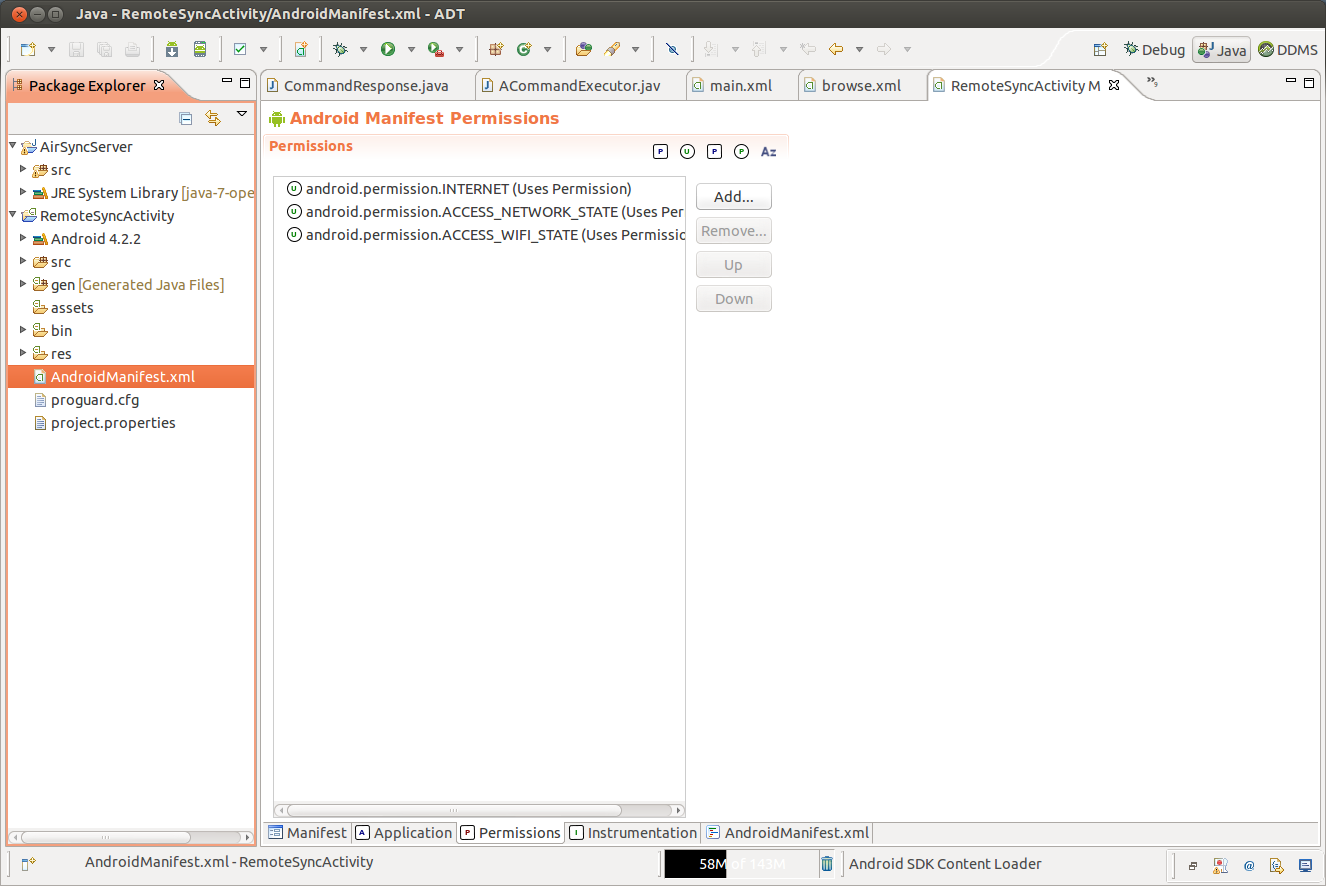
\includegraphics[width=1\textwidth]{permissions.png}
\caption{Android Activity Permissions Editor}
\end{figure}

\item Android does not allow some SystemIO calls to occur from the primary thread of an Activity.  I ran into this problem with Socket IO. Similarly, when attempting to change the current application view from  The non-descriptive RuntimeException below was being thrown whenever I tried. I was unable to find documentation of this on androids development site, but with trial and error discovered that it worked fine in a separate thread. My assumption as that Android does this to avoid causing the interface to hang or lock up while waiting for SystemIO. 
\begin{figure}[H]
\center
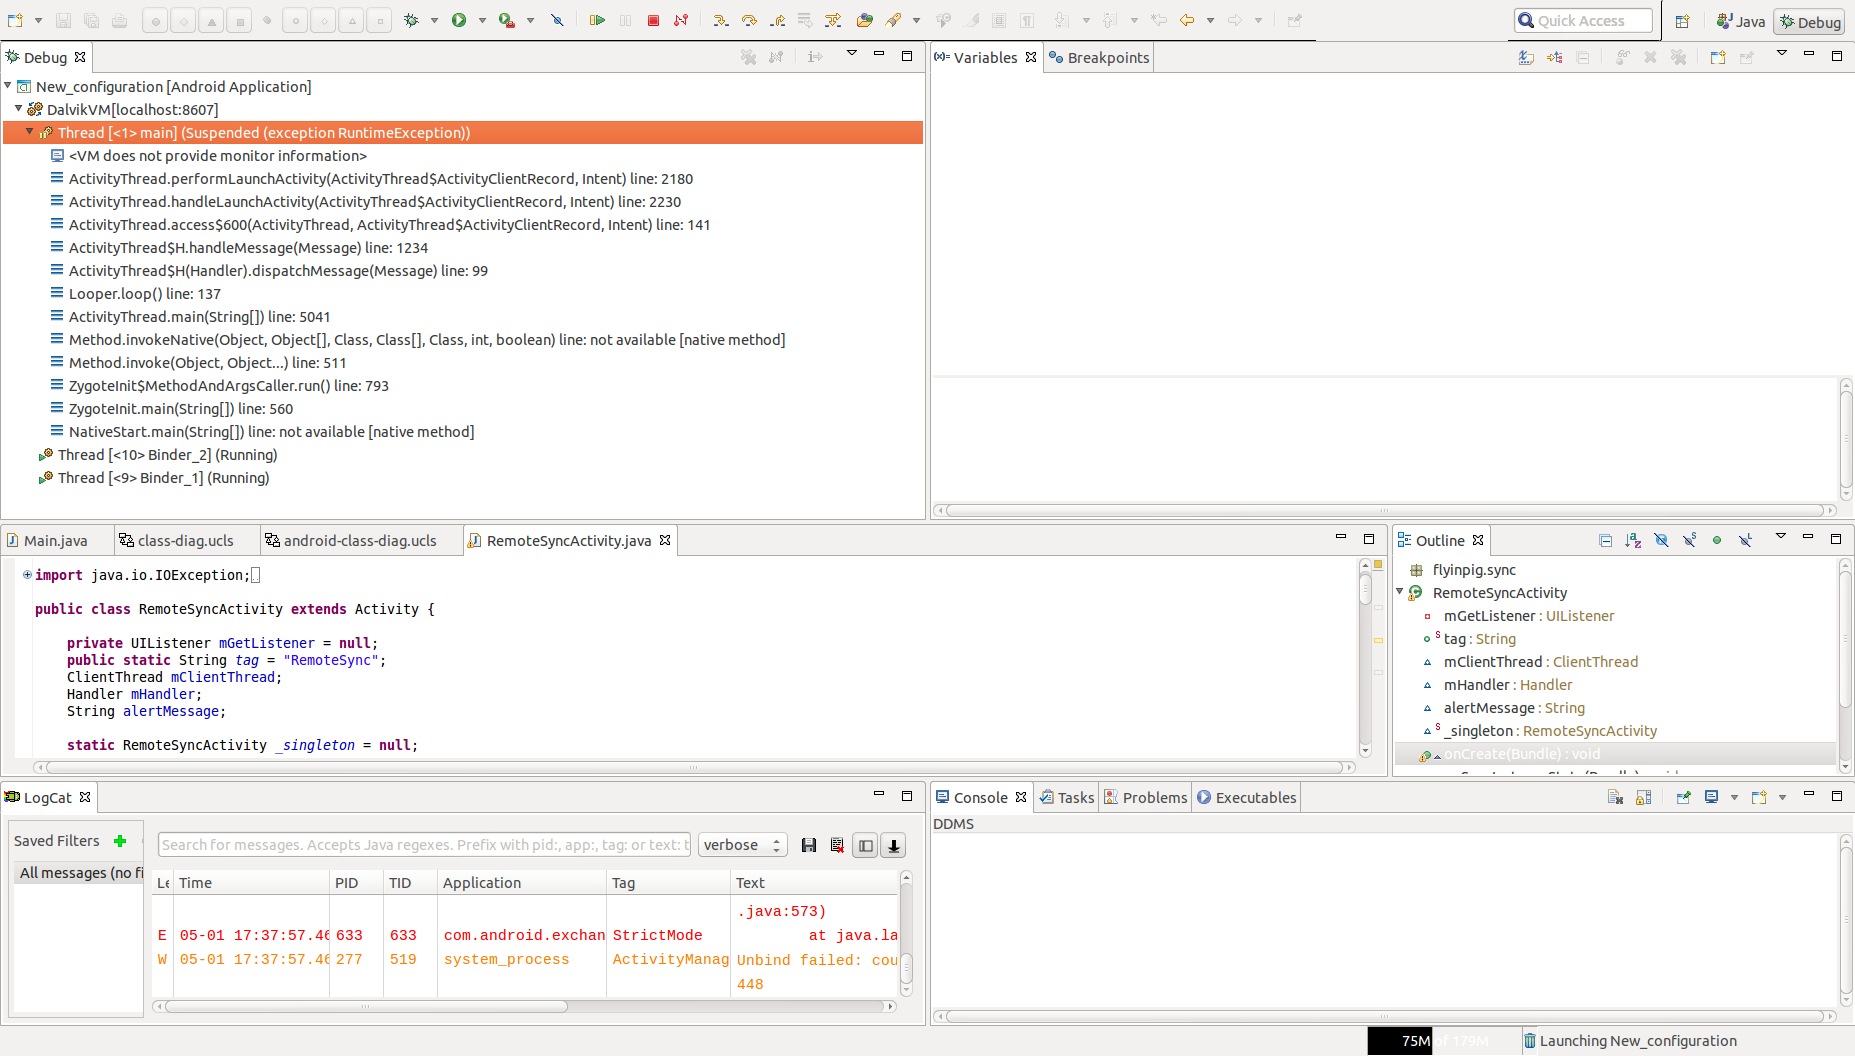
\includegraphics[width=1\textwidth]{runtimeexception.png}
\caption{Non-descriptive RuntimeException}
\end{figure}

\item Android also uses XML files to define graphical user interface(GUI) layout. In Java GUIs are defined in the source code, which is typically defining buttons,text labels, fields, etc. and there locations. By moving this definition to XML files called Views or Layouts it significantly cleans up the associated code. In this project I only need to attached Listeners to the Views that I created. I only used the onClick Listener for this project. View object likes buttons are clickable by default, but other view objects like TextView (The equivalent to a JLabel in java) must be specified as follows within its XML definition.
\begin{center}
\begin{tabular}{|l|}
\hline
\emph{    android:onClick="onClick"}\\  
\emph{    android:clickable="true"}\\
\hline
\end{tabular}
\end{center}

\begin{figure}[H]
\center
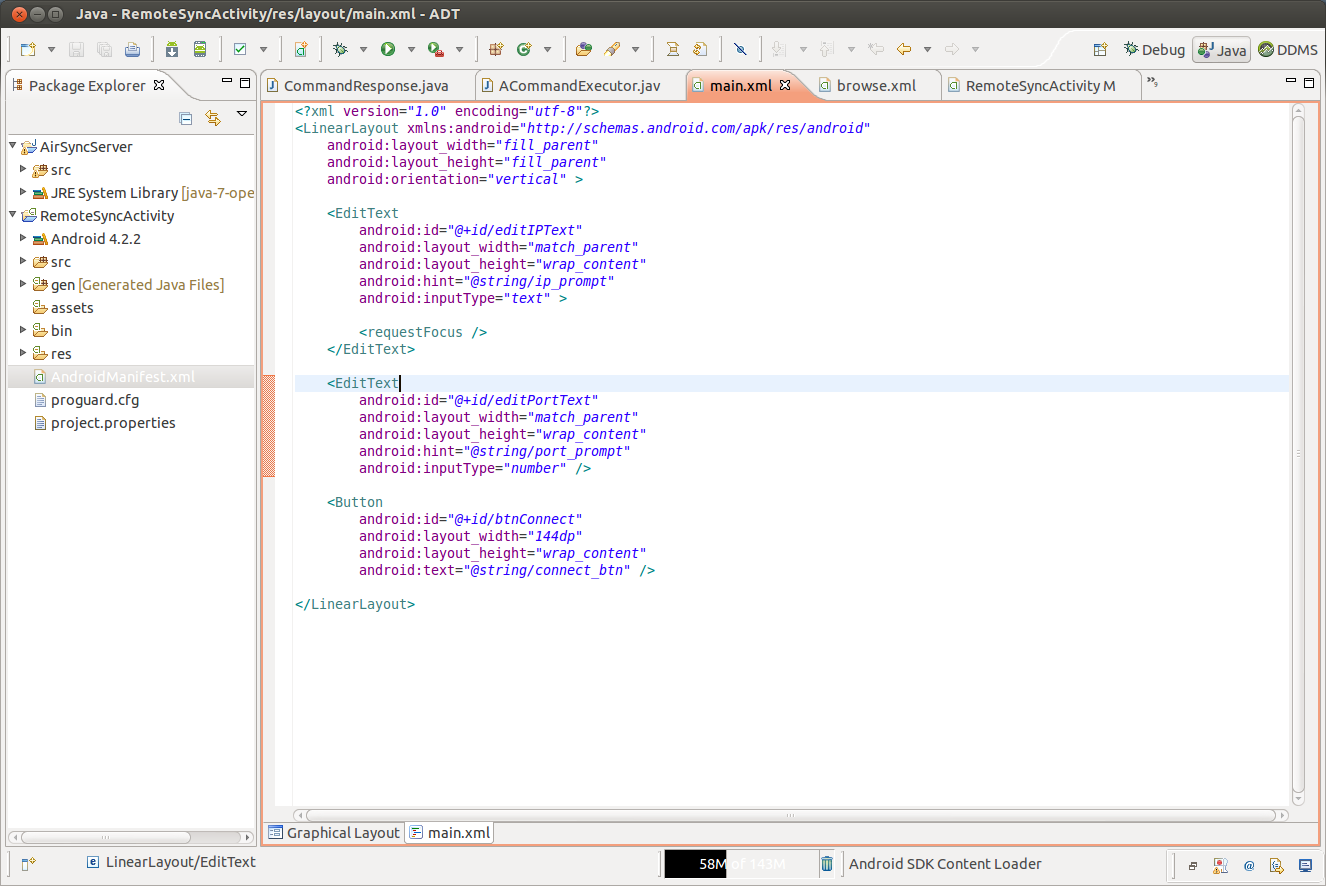
\includegraphics[width=1\textwidth]{view-xml.png}
\caption{Android View/Layout XML}
\end{figure}

\item The ADT provides a set of emulators that can be configured to matched the desired device specifications and Android versions. This provides an simple method for a developer to try an application on a broad set of configurations. During my development I noticed that system calls that collected information about the device did not behave consistently in the emulator and was causing errors. I was unable to isolate the exact problem, but the same code that failed in the emulator worked well on both physical devices I tried.  Some forum posts I read indicated other developers were having similar finicky issues with the emulated devices.

\end{itemize}

Android applications are strictly structured as \emph{Activities} or \emph{Services}. I developed this application as an activity, which provides the user interaction performs actions when the the application is active.\\
\\
Although the android development libraries are very similar to the standard Oracle Java Runtime libraries, I found a few discrepencies in how Oracle Java libraries when compared to Android. One in particular is related to Input/Output. DataInputStream and DataOutputStream functions to read and write UTF Strings to the network do not seem to be compatible when attempting to use the Android and Oracle versions together. In this case I wrote compatible replacement code using readChar() as a work-around.\\

\section{Conclusion}

I intend to continue developing this project for personal use and with the intent to share the source code and allow open development. With the adition of access control restrictions and encrypted communication this is the a document and media sharing solution that can provide corporations and individuals with the benefits of cloud sharing without the privacy concerns. Where corporations can own the assets and allow employees to access work documents on mobile devices securely.  
\end{document}